\documentclass[11pt,sigconf]{iabart}
%\documentclass[10pt,sigconf,letterpaper]{acmart}
%\usepackage[vskip=1em,font=itshape,leftmargin=2em,rightmargin=2em]{quoting}
\usepackage[skip=4pt plus1pt]{parskip}
%\copyrightyear{2024}
%\acmYear{2024}
%\setcopyright{acmlicensed}\acmConference[IAB Network Management WS]{The IAB Next Era of Network Management Operations}{December 3, 2024}{}
%\acmBooktitle{The IAB next Era of Network Management Workshop}{December 3, 2024}{}

\begin{document}

\title{Managing IoT Devices with LwM2M}


\author{Jaime Jiménez}
\email{jaime.jimenez@ericsson.com}
\orcid{0009-0008-2864-4269}
\affiliation{%
  \institution{Ericsson}
  \city{Jorvas}
  \country{Finland}
}

\begin{abstract}

In this paper we provide an overview of the Lightweight Machine-to-Machine (LwM2M) protocol, a standard device and service management protocol built on top of CoAP for remote management and configuration of devices. We highlight its role in IoT device management and its use of key IETF standards such as CoAP, DTLS,and OSCORE. While network management protocols like SNMP, RESTCONF, and CORECONF focus on monitoring and configuring endpoints within the network, LwM2M extends these capabilities by managing the entire lifecycle of individual devices, including configuration, control, and maintenance. We also discuss LwM2M's architecture, data model and communication interfaces. Last, we also introduce recent advancements in the protocol.

\end{abstract}

\keywords{Internet of Things, IoT, network management, device management, security, standards}

\maketitle

\section{Introduction} \label{introduction}

The rapid evolution of network management protocols necessitates a reevaluation of existing technologies and their applicability to modern challenges. The Lightweight Machine-to-Machine (LwM2M) protocol~\cite{lwm2m-spec}, developed by the Open Mobile Alliance (OMA), is a key player in this domain, offering a standardized framework for managing Internet of Things (IoT) devices~\cite{oma-sdo}. This paper explores the role of LwM2M in the context of the IAB workshop on the Next Era of Network Management Operations, focusing on its current deployments, challenges, and future potential.

The IAB "NEMOPS" workshop seeks contributions that critically assess the progress made since the 2002 IAB workshop, particularly in terms of network management protocols. This paper aims to present LwM2M, an management protocol that addresses the needs for managing IoT endpoints from the operational point of view of device and network management.

Our contribution is informed by the authors' extensive experience with IoT and contributions in the IoT domain both at IETF and in OMA. The rest of the document is organized as follows: The \hyperref[introduction]{Introduction} outlines LwM2M as a standardized framework for managing IoT devices, addressing current network management challenges. The \hyperref[overview]{LwM2M Protocol Overview} details its architecture, focusing on communication between Clients, Servers, and Bootstrap Servers (see Figure~\ref{fig:overall_architecture}). Recent advancements, including integrations with blockchain and industrial protocols, are discussed in \hyperref[extensions]{LwM2M Extensions}, the \hyperref[conclusions]{Conclusions} summarize the main points of the paper.

\textbf{LwM2M and IETF}

The IETF has played a fundamental role in shaping the protocols that underpin LwM2M. IETF efforts have focused on adapting existing Internet and Web protocols to meet the needs of resource-constrained IoT devices ~\cite{9139045}.

LwM2M is built upon several key IETF standards. At the core is the \textit{Constrained Application Protocol (CoAP)}~\cite{rfc7252}, a lightweight RESTful protocol designed for constrained environments, providing the fundamental request/response model for LwM2M communications. \textit{RFC 7959}~\cite{rfc7959} defines block-wise transfers in CoAP, allowing LwM2M to efficiently handle large payloads by breaking them into smaller blocks. The \textit{LwM2M} protocol also leverages \textit{RFC 7641}~\cite{rfc7641} for resource observation, enabling clients to subscribe to changes of resource state without continuous polling. For secure communications, LwM2M often relies on the \textit{Datagram Transport Layer Security (DTLS)} as outlined in \textit{RFC 6347}~\cite{rfc6347}, ensuring encryption and integrity over the CoAP protocol. An alternative layer of security is provided by \textit{Object Security for Constrained RESTful Environments (OSCORE)}~\cite{rfc8613}, which offers end-to-end encryption and integrity protection directly at the application layer, making it suitable for scenarios where DTLS is not applicable. Lastly the \textit{Constrained RESTful Environments (CoRE) Resource Directory (RD)}~\cite{rfc9176} facilitates resource registration of IoT endpoints. It does so by maintaining information about resources on other servers, the lookup interface, although present is not intended for applications but solely for management purposes.
\sloppy

LwM2M also supports additional transport protocols, such as IETF's \textit{Hypertext Transfer Protocol (HTTP)}\cite{http-spec} and OASIS' \textit{Message Queuing Telemetry Transport (MQTT)}\cite{mqtt-spec}, expanding its applicability across diverse network environments and use cases.

\section{LwM2M Protocol Overview} \label{overview}

\begin{figure}[h]
  \centering
  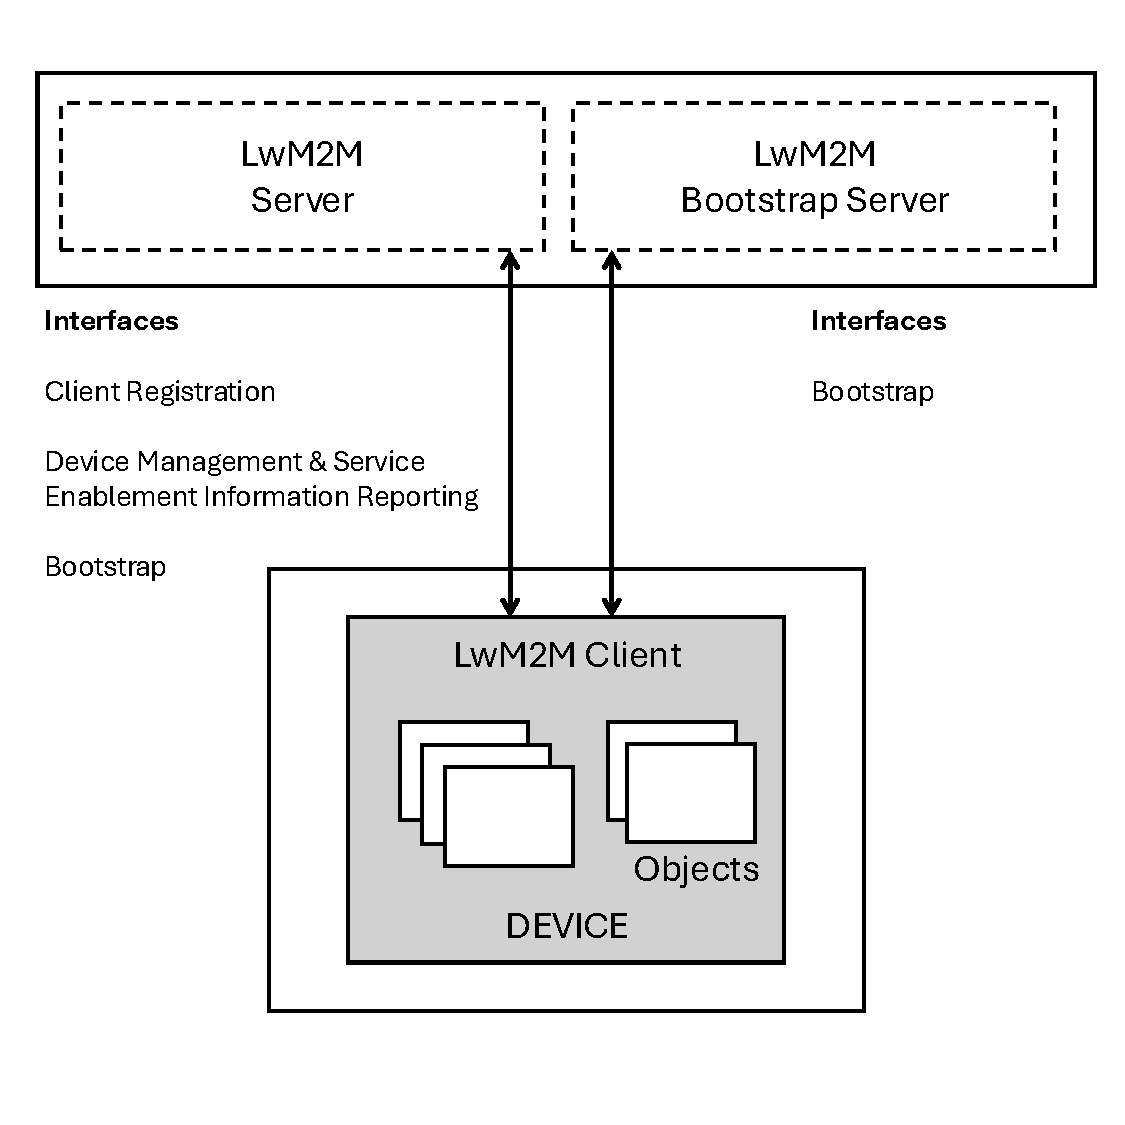
\includegraphics[width=0.5\textwidth]{figs/arch.pdf}
  \caption{General LwM2M Architecture}
  \label{fig:overall_architecture}
\end{figure}

This section presents an overview of the LwM2M protocol, emphasizing its participating entities, data model, and communication interfaces.

\textbf{Participating Entities}

The LwM2M protocol defines three primary entities that form the backbone of its communication architecture:

\begin{itemize}
  \item \textbf{LwM2M Client}: Typically a smart device, such as a light, smart meter, switch, or gateway, responsible for data collection and resource management at the device level. The client oversees the lifecycle of various objects residing in it and communicates with servers to transmit data and receive management instructions.
  \item \textbf{LwM2M Server}: Often referred to as the manager, this server manages multiple clients, aggregates their data, and issues configuration or maintenance commands. It is essential for controlling and coordinating client devices within an IoT ecosystem.
  \item \textbf{LwM2M Bootstrap Server}: This entity is responsible for the initial configuration of the LwM2M Client. Unlike other protocols, LwM2M includes a Bootstrap Server to streamline device setup, particularly when multiple servers are involved. During the bootstrap process, it provides the client with configuration details, such as security credentials and connection information, which can be pre-integrated into the device's software or dynamically supplied by the Bootstrap Server.
\end{itemize}

The introduction of the Bootstrap Server differentiates LwM2M from other IoT protocols. Before the client can establish a connection to a server, it undergoes the bootstrap procedure to load initial configurations and key material. This feature is particularly advantageous in scenarios with multiple servers or when load balancing is required, as it allows for flexible and dynamic configuration.

\textbf{LwM2M Data Model}

The LwM2M protocol employs a structured, object-based data model to facilitate communication between clients and servers. In this model, each data entity is defined as an object, uniquely identified by an integer ID, as specified by the Open Mobile Alliance (OMA). These objects can represent various resources, such as sensors, actuators, or configuration settings.

Each object consists of multiple resources, which serve as the fundamental data points within the object. Resources are assigned integer IDs and are classified as either mandatory or optional, depending on the object's intended function being the mandatory ones used for interoperability purposes. An object can also have multiple instances, each with a unique instance ID, allowing for flexibility. For instance, a device with several sensors can represent each sensor as an instance of the same object, such as in a network of connected lightbulbs.

The LwM2M data model enables servers to access individual resources, instances, or entire objects using well-defined URI strings. The URI template approach follows the Web Linking and the IETF CoRE Link Format~\cite{rfc6690}. The format is as follows:
\[
/<Object ID>/<Instance ID>/<Resource ID>
\]
In this structure, the instance or resource ID can be omitted if the request targets the entire object or a specific instance. This model provides a straightforward way to interact with data at different levels of granularity.

All objects are listed in the LwM2M Registry~\cite{lwm2m-registry}, categorized as either application-oriented (e.g., thermostats, lamps) or system-oriented (e.g., security, connectivity). Those for applications follow the same schema and come from the IP for Smart Objects (IPSO)~\cite{ipso} consortium which was integrated into OMA. 

\textbf{Communication Interfaces}

LwM2M defines four primary communication interfaces that facilitate interactions between clients and servers, each serving distinct roles in the protocol's operation:

\begin{itemize}
  \item \textbf{Bootstrap Interface}: This interface facilitates the initial setup by enabling the client to obtain necessary configurations and security credentials from the Bootstrap Server prior to connecting with an LwM2M Server. The process can be either automated or client-initiated.
  
  \item \textbf{Registration Interface}: After the bootstrap procedure, the client registers with the LwM2M Server through the Registration Interface. During registration, the client provides its endpoint name whcih together with the security credentials is used as identifier. To maintain its registration status, the client must periodically send updates. If these updates are not received within the agreed time, the client is considered de-registered and must re-initiate the registration process.
  
  \item \textbf{Device Management and Service Enablement Interface}: Once registered, the server can use this interface to perform various management tasks, such as reading and writing data or executing commands on the client. It allows the server to control the client's resources, adjusting settings or triggering actions as required.
  
  \item \textbf{Information Reporting Interface}: This interface enables the client to report changes in its status or resource values to the server, using the Observe function. The server can set up observation requests, prompting the client to notify it when certain resource values change or when predefined conditions are met. This capability is particularly useful for monitoring dynamic IoT environments where timely updates are crucial. LwM2M defines specific attributes to configure how frequently these notifications occur.
\end{itemize}

LwM2M has been integrated on most IoT OSs like FreeRTOS~\cite{freertos}, Mbed~\cite{mbed}, RIOT OS~\cite{riot_os}, Contiki-NG~\cite{contiki_ng}, and many others, with a strong focus on IoT device security~\cite{pop00010}.

LwM2M has also proven to be a preferred solution for managing cellular IoT (CIoT) devices~\cite{10333286} due to its low overhead and comprehensive management capabilities, particularly in environments where network efficiency, scalability, and efficient firmware updates are critical~\cite{8725488}.

\section{LwM2M Evolution} \label{extensions}

LwM2M, though robust in its core functionalities, has advanced through various extensions and integrations. This section explores a subset of recent research developments that may inspire the future evolution of the standard.

Firstly, LwM2M has developed a Northbound Web API to simplify interaction with LwM2M systems by abstracting the protocol's complexities~\cite{lwm2m-northbound-api}. This API enables external applications to perform key operations such as tracking device registrations, executing management commands (e.g., read, write, delete), and subscribing to observations for real-time monitoring of device resources.

Outside OMA, several studies have concentrated on enhancing IoT security through the use of LwM2M. For instance, Muhammad et al.~\cite{pop00001} investigated the use of ARIA cryptography within Hardware Secure Modules for both LwM2M and MQTT protocols. Similarly, Lanzieri et al.~\cite{pop00011} proposed extensions to the LwM2M core specification to facilitate secure and authorized client-to-client communication, which is a limitation of the current standard.

Others have focused on interoperability between SDOs, Kim et al.~\cite{pop00007} have designed and implemented a blockchain-based system that enables interworking between oneM2M~\cite{oneM2M-spec} and LwM2M IoT systems. Their approach uses blockchain's immutable and distributed ledger properties for interoperability and security. 

In the context of Industrial IoT (IIoT), Yaker et al.~\cite{pop00004} introduced a novel edge Security Information and Event Management (SIEM) system for managing IoT flows within 5G private networks. Their approach incorporates LwM2M data events to manage and secure IoT data in a 5G environment. Similarly, Myoung et al.~\cite{pop00012} addressed the integration of LwM2M with smart metering technologies, proposing a data interworking model between the Device Language Message Specification (DLMS)~\cite{dlms-spec} used for managing smart meters and the LwM2M protocol.

Further efforts have been made to integrate LwM2M with industrial communication protocols. Karaagac et al.~\cite{pop00013} explored the interoperability between LwM2M and the Open Platform Communications Unified Architecture (OPC UA), proposing a framework where OPC UA Servers can be virtualized as LwM2M Clients and vice versa. Similarly, Cavalcanti et al.~\cite{pop00014} reviewed various machine-to-machine communication protocols within the context of Industry 4.0. A third example is based only on CoAP, Wang et al.~\cite{pop00015}, which proposed a CoAP-based OPC UA transmission scheme tailored for resource-constrained devices. These three papers aim to bridge the gap between IoT and industrial automation.

The evolution of LwM2M has also prompted considerations for enhancing its data model capabilities. While the current IPSO data model, utilizing the format \textit{/<ObjectID>/<InstanceID>/<ResourceID>}, is well-suited for constrained environments, it may fall short in addressing the needs of complex machines or network nodes with large, deeply nested configuration structures. This limitation suggests the potential for developing alternative data models that can accommodate more intricate configurations, thereby extending the LwM2M protocol's applicability to a broader range of devices.

The interoperability of LwM2M with hyperscalers is hindered by the lack of native CoAP support within these platforms. This limitation poses a challenge for vendors seeking to integrate LwM2M-based IoT solutions with HCS services. To overcome this obstacle, some vendors have devised methods to encapsulate CoAP messages within MQTT topics, although this solution is merely a workaround that may not fully address the efficiency needs of large-scale IoT deployments.

\section{Conclusions} \label{conclusions}

This paper provides an overview of the LwM2M protocol, detailing its core components, architecture, and integration with IETF standards. We explored its role in managing IoT devices, including its communication interfaces and data model, and discussed its adaptability through recent extensions. LwM2M continues to evolve as a key solution for IoT device management, offering scalability, security, and efficient operation, especially in constrained environments like Cellular IoT (CIoT). Future developments in interoperability and security enhancements will further strengthen its utility across diverse IoT applications.

\section{Acknowledgments}

We would like to thank Ericsson for their support of this work. Special thanks to Jari Arkko, Carsten Bormann and Sándor Katona for their valuable review and feedback, which improved the quality of this paper.

\bibliographystyle{ACM-Reference-Format}
\bibliography{paper}

\end{document}
\endinput
